\documentclass[10pt]{article}
\usepackage[a4paper,margin=2cm]{geometry}
\usepackage[T1]{fontenc}
\usepackage{lmodern}
\usepackage{graphicx}
\usepackage{booktabs}
\usepackage{amsmath}
\usepackage[hidelinks]{hyperref}
\usepackage{caption}
\captionsetup{font=small,labelfont=bf}
\setlength{\parskip}{3pt}

\title{Can we tell from physiology when someone is stressed by a video?\\
Detecting self-reported stress reactions in new people and new videos}
\author{Mathias Chebbah, Team 12\\\small HABS Neuro-AI Hackathon, Universit\'e Paris-Saclay, November 2026}
\date{}

\begin{document}
\maketitle

\begin{abstract}
The HABS dataset has no stress measure, so we used each participant's own
ratings: a trial counts as a stress reaction when it was rated negative and
activating. We asked whether EEG, heart, skin and breathing signals recorded
during a 10-second video can detect these reactions in people and video themes
the model never saw, and which signals change. Across 15,055 development
trials we ran 43 model variants, including eleven scikit-learn model families,
and the within-person AUC rose from 0.537 to 0.585. On a sealed test opened
once, the final model reached 0.605 (95\% interval 0.544 to 0.668) for new
people watching new themes, and 0.592 and 0.561 in the two larger test
regimes. The starting model did as well (0.634, 0.588, 0.555), so the gains we
found during the search did not hold up. Detection is above chance but weak.
Separating stress from excitement at equal arousal was unreliable (0.45 to
0.59 depending on the test set), while stress versus relaxed held at 0.61 to
0.63. The physiology is consistent across contrasts: stressful trials come
with lower relative alpha power, larger skin conductance responses, shallower
breathing and a slower, not faster, heart rate, the cardiac deceleration known
from aversive picture viewing.
\end{abstract}

\section{Why we asked this}

Acute stress shows up in the body before anyone says a word: the heart speeds
up, the skin sweats, breathing changes, and EEG rhythms shift. In jobs where
people work under pressure, such as surgery, being able to read this from
sensors would be useful. Our team includes a physician, and that is where the
question came from. The HABS dataset records 64-channel EEG, ECG, skin
conductance and breathing while 314 people watch short emotional videos and
rate each one. It has no stress questionnaire, no cortisol and no stress task,
so we used what it does have: after each video, people rate how negative and
how activating it felt. Giannakakis et al.\ (2015) used the same idea on
self-rated video trials to separate stress from relaxed states.

Two problems make this harder than it looks. First, the same videos come back
for many participants, and a recent HABS preprint showed that emotion decoders
can end up recognising the video instead of the person's state. Second, a
stress detector could just be an arousal detector, since excitement also
speeds the heart and makes the skin sweat. We designed the study around both
problems.

\section{What we did}

\paragraph{Labels.} We call a trial a \emph{stress reaction} when the
participant rated it negative (valence $\le 4$ on 1 to 9) and activating
(arousal $\ge 6$). Everything else is "not stressed". This is a self-reported,
acute reaction to a video, in healthy volunteers. To check what the detector
picks up, we fixed three control contrasts before looking at any result:
stress versus excitement (arousal $\ge 6$, valence $\le 4$ versus $\ge 6$),
stress versus calm negative (valence $\le 4$, arousal $\ge 6$ versus $\le 4$),
and stress versus relaxed (valence $\ge 6$, arousal $\le 4$), the contrast of
Giannakakis et al.

\paragraph{Features.} One job on the HABS GPU servers computed, for each of
the 22,974 audited trials, log band power (1 to 45 Hz, five bands) on every EEG
channel during the 10-second video and the 2 seconds before, short evoked
responses, a 20-channel covariance, and body signals. Following the mentors'
suggestion to compute heart rate variability on windows shorter than the usual
30 seconds, we computed it on the 10-second video itself: mean RR interval,
RMSSD, SDNN and the change in heart rate from the 5 seconds before. For the
skin we measured the event-related conductance rise 1 to 6 seconds after
onset, the number of responses and the steepest rise. For breathing we
measured rate, change in rate, depth, irregularity and the longest pause. We
left out eye tracking, which the organisers reported as misaligned.

\paragraph{Splits and score.} We hash every participant and every video theme into five
buckets with a salt specific to this study, so its test set differs from our
previous study's. Bucket 0 of both is the sealed test (new person, new theme;
818 trials, 60 people, 18 themes). Two larger test sets overlap with it: test
people with the other themes (3,194 trials) and the other people with the test
themes (3,907 trials). The remaining 15,055 trials (254 people, 66 themes) are
the development set, scored by a $3\times3$ cross-fit in which every block is
predicted by a model trained on other people and other themes. The video
name, theme, intended emotion and start marker are hidden from the rows being
predicted. The score is the area under the ROC curve computed inside each
person who has at least three stressed and three other trials, averaged over
people. Chance is 0.5, and a person's general physiology or rating habits
cannot raise it. In development, 23\% of trials were stress reactions.

\paragraph{Model search.} The scoring code stayed fixed and we only edited one
model file. A GitHub Actions job took the model file from each experiment
commit and the rest from \texttt{main}, so no variant could change how it was
scored, and only aggregate numbers left the runner. We scored variants in
parallel batches and kept one only when it beat the best development score by
at least 0.005; ablations were logged but never kept. We opened the sealed test
once, at the end.

\paragraph{Correlates.} On development data only, for each person with at
least three trials in both groups, we computed the standardised difference
(Cohen's $d$, using that person's pooled standard deviation) of each feature
between stressed and other trials, then averaged over people with a 95\%
bootstrap interval. We did the same for the control contrasts.

\section{Results}

\paragraph{The search.} Figure~\ref{fig:progress} shows all 43 experiments.
The starting model, a logistic regression on channel-level band power and body
summaries, scored 0.537. Adding the short-window heart, skin and breathing
features alone gave 0.541. The biggest step came from predicting valence and
arousal separately with ridge regressions on person-centred ratings and
scoring stress as predicted arousal minus predicted valence (0.578). Centring
every feature on the person's own mean brought 0.585, and keeping only the
regional view gave the same score with one regression per rating instead of
two. We then tried eleven scikit-learn families on the same task:
partial least squares (0.580), an RBF kernel (0.574), linear SVR (0.572), a
small MLP (0.571), Huber regression (0.571), a linear SVM classifier (0.565),
random forest (0.563), shrinkage LDA (0.560), extra trees (0.558), gradient
boosting (0.555) and nearest neighbours (0.545). None beat the ridge.
Weighting valence and arousal differently, an "and" rule, frontal asymmetry,
evoked responses and pre-video baselines did not help either, and we stopped
after two batches without a kept change.

\begin{figure}[t]
\centering
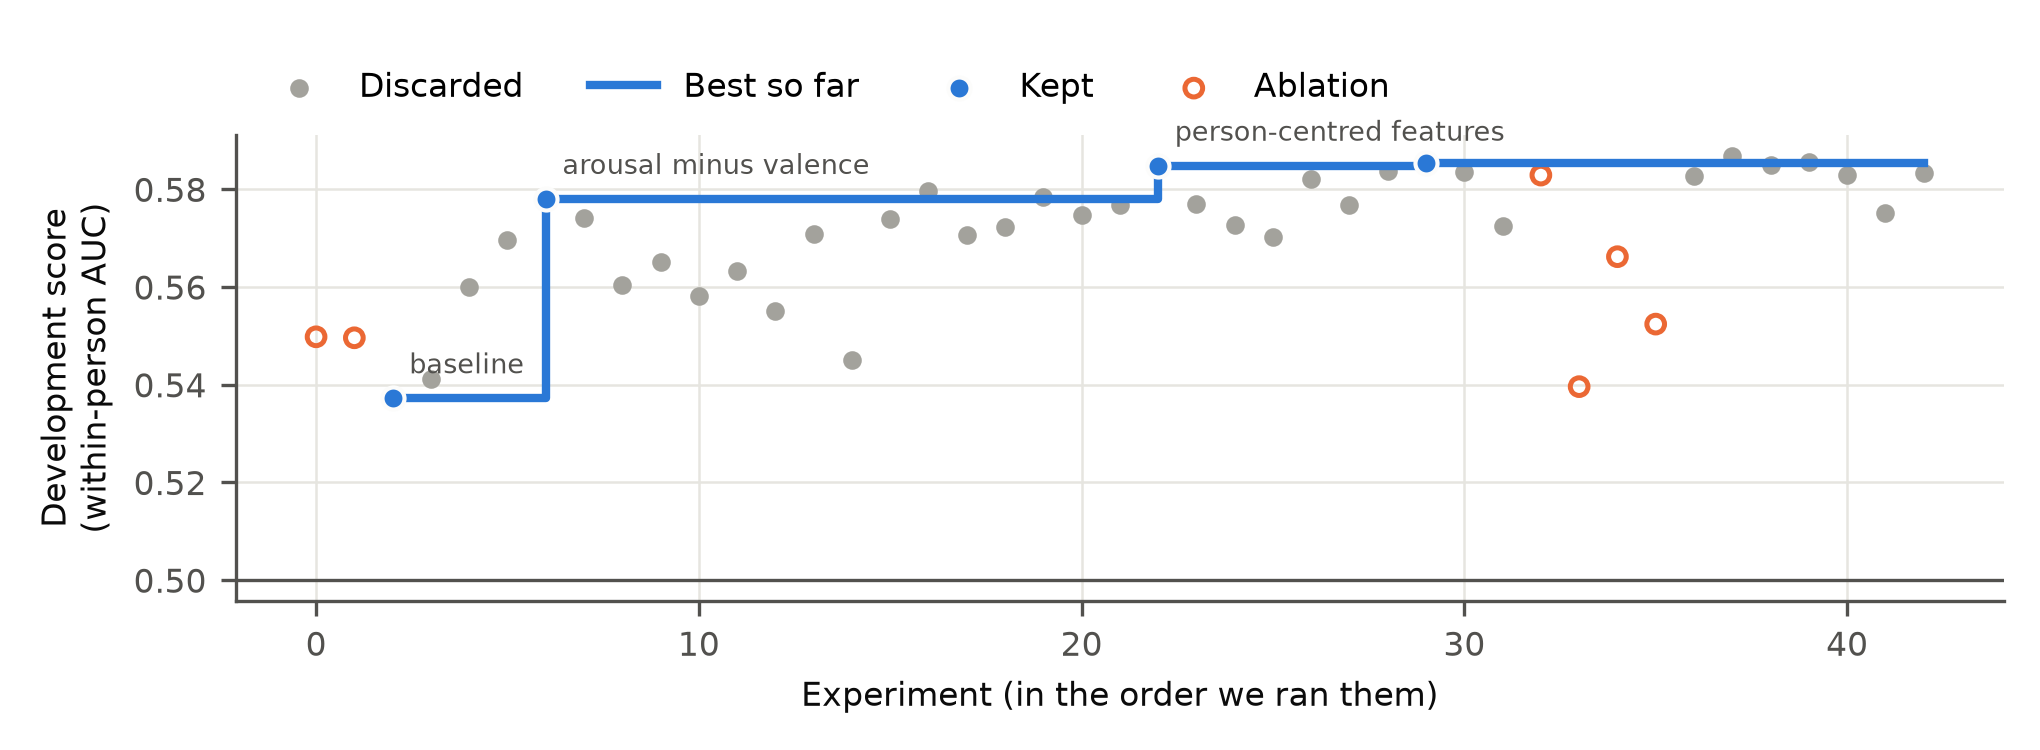
\includegraphics[width=\linewidth]{figures/progress.png}
\caption{Development score of the 43 experiments in the order we ran them.
Blue points are kept changes and the line is the best score so far. Open
orange circles are ablations.}
\label{fig:progress}
\end{figure}

\paragraph{The sealed test.} Table~\ref{tab:test} and
Figure~\ref{fig:test} give the results. Every model detects stress reactions
above chance in new people, with intervals that exclude 0.5 in the two regimes
that have new people. The final model was not better than the starting model.
In the primary regime the paired difference was $-$0.029 ($-$0.069 to
+0.008), and in the larger regimes +0.004 ($-$0.020 to +0.029) and +0.006
($-$0.018 to +0.029). The development gain of +0.048 did not survive the test.
Only 35 of the 60 primary test people had enough trials of both kinds, so
those intervals are wide, but the two larger regimes tell the same story.

\begin{table}[t]
\centering
\small
\begin{tabular}{lccc}
\toprule
 & New person, new theme & New person, seen theme & Seen person, new theme\\
 & 35 people & 55 people & 136 people\\
\midrule
Starting model & 0.634 [0.570, 0.699] & 0.588 [0.561, 0.615] & 0.555 [0.524, 0.586]\\
Final model & 0.605 [0.544, 0.668] & 0.592 [0.563, 0.621] & 0.561 [0.531, 0.590]\\
\quad EEG only & 0.603 [0.539, 0.666] & 0.586 [0.559, 0.613] & 0.560 [0.529, 0.591]\\
\quad Body only & 0.541 [0.491, 0.595] & 0.545 [0.514, 0.577] & 0.545 [0.515, 0.574]\\
\midrule
Final, stress vs excitement & 0.448 (10 people) & 0.586 (51) & 0.519 (41)\\
Final, stress vs calm negative & 0.683 (10) & 0.559 (31) & 0.594 (45)\\
Final, stress vs relaxed & 0.633 (20) & 0.629 (49) & 0.612 (77)\\
Final, pooled AUC & 0.595 & 0.578 & 0.559\\
\bottomrule
\end{tabular}
\caption{Sealed-test within-person AUC with 95\% intervals from resampling
people. People are counted when they have at least three trials of each kind.
All models were fitted once on the development trials.}
\label{tab:test}
\end{table}

\begin{figure}[t]
\centering
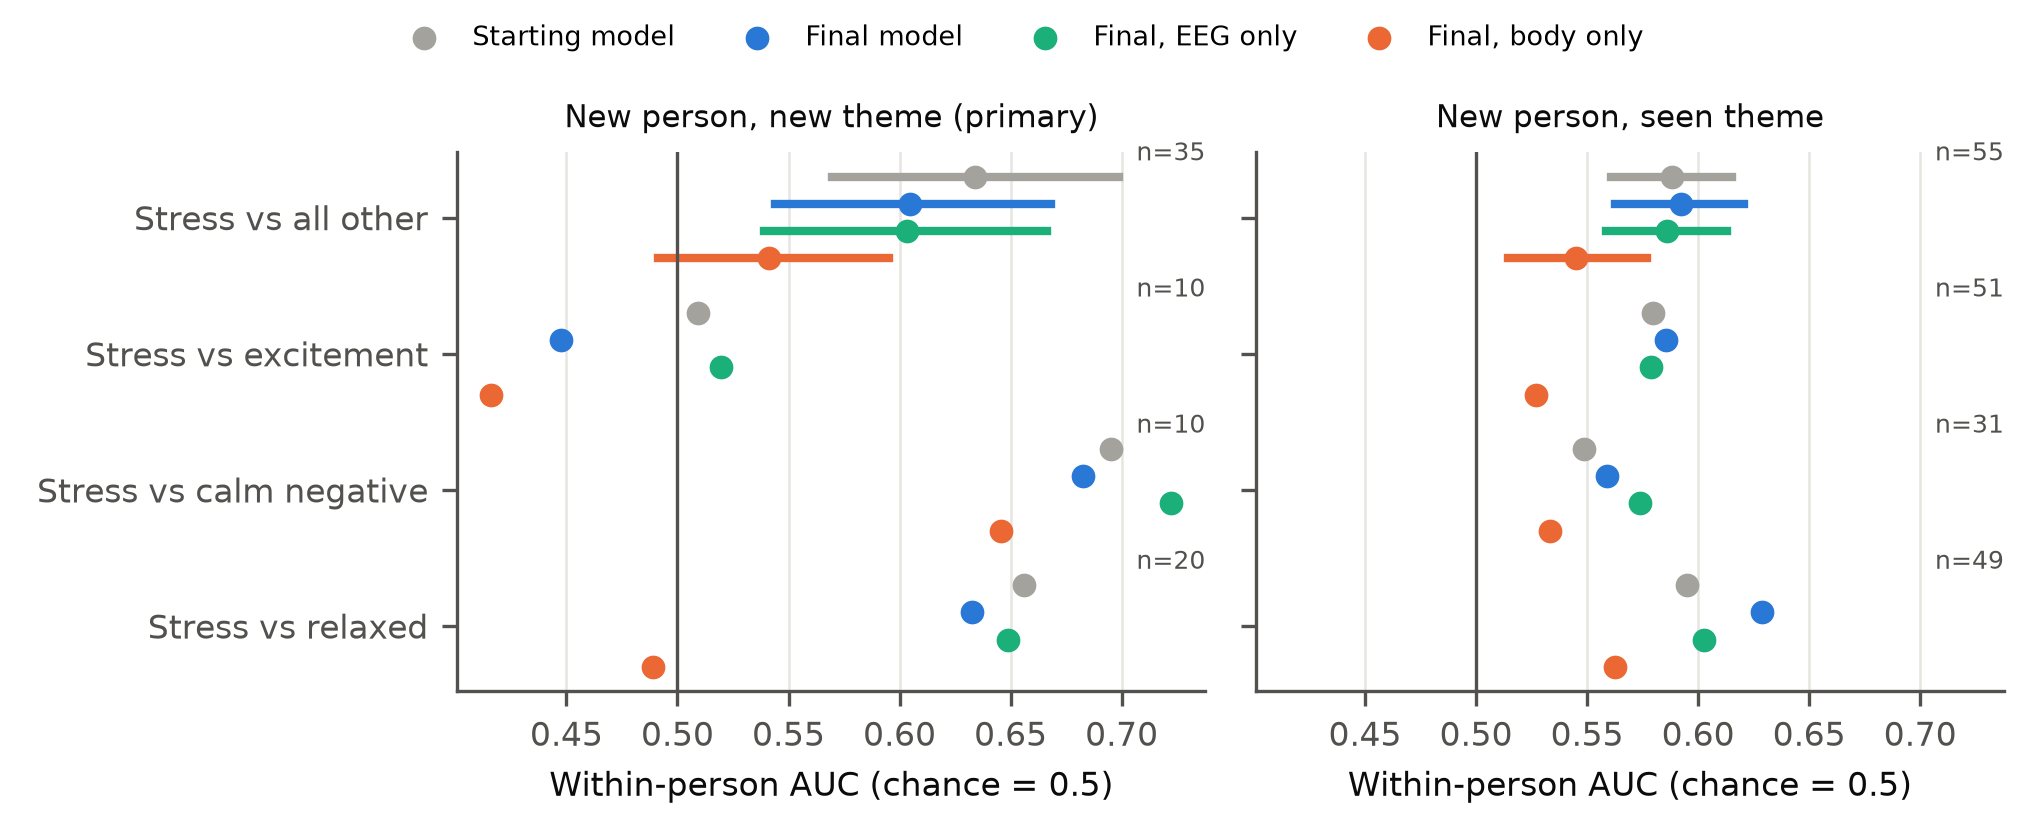
\includegraphics[width=\linewidth]{figures/sealed_test.png}
\caption{Sealed-test AUC for the main score and the three control contrasts,
in the two regimes with new people. Bars are 95\% intervals for the main
score; $n$ is the number of people with enough trials of both kinds.}
\label{fig:test}
\end{figure}

\paragraph{Stress or just arousal?} At equal high arousal, telling stress from
excitement was unreliable on the test set: 0.586 with 51 people, 0.519 with
41, and 0.448 with only 10. Stress versus relaxed, the contrast of Giannakakis
et al., held between 0.61 and 0.63 in all three regimes. EEG alone did almost
as well as the full model, while heart, skin and breathing alone stayed near
0.54 and close to chance against excitement. The body signals mostly carry
activation; whatever separates stress from excitement is in the EEG, and it
is weak.

\paragraph{What changes in the body and the brain.}
Figures~\ref{fig:eeg} and \ref{fig:body} show the within-person effect sizes
in development. On stressed trials, relative alpha power was lower over the
whole scalp ($d$ from $-$0.20 to $-$0.25), relative delta was higher over
frontal sites (+0.21), the skin conductance rise 1 to 6 s after onset was
larger (+0.20), breathing was shallower ($-$0.12), and heart rate was lower
($-$0.12) and dropped relative to the 5 seconds before the video ($-$0.11). The
heart slows down: this is the cardiac deceleration reported for unpleasant
pictures and films, not the speeding-up people usually picture for stress. The
deceleration and the skin response remained against excitement ($-$0.17 and
+0.14), and the alpha decrease was strongest against calm negative trials,
which fits alpha suppression as an activation marker. The 10-second heart
measures matched the earlier heart-rate estimate ($r$ = 0.94 over 9,643
trials) and were available for 93\% of trials, against 65\% for the older
estimate.

\begin{figure}[t]
\centering
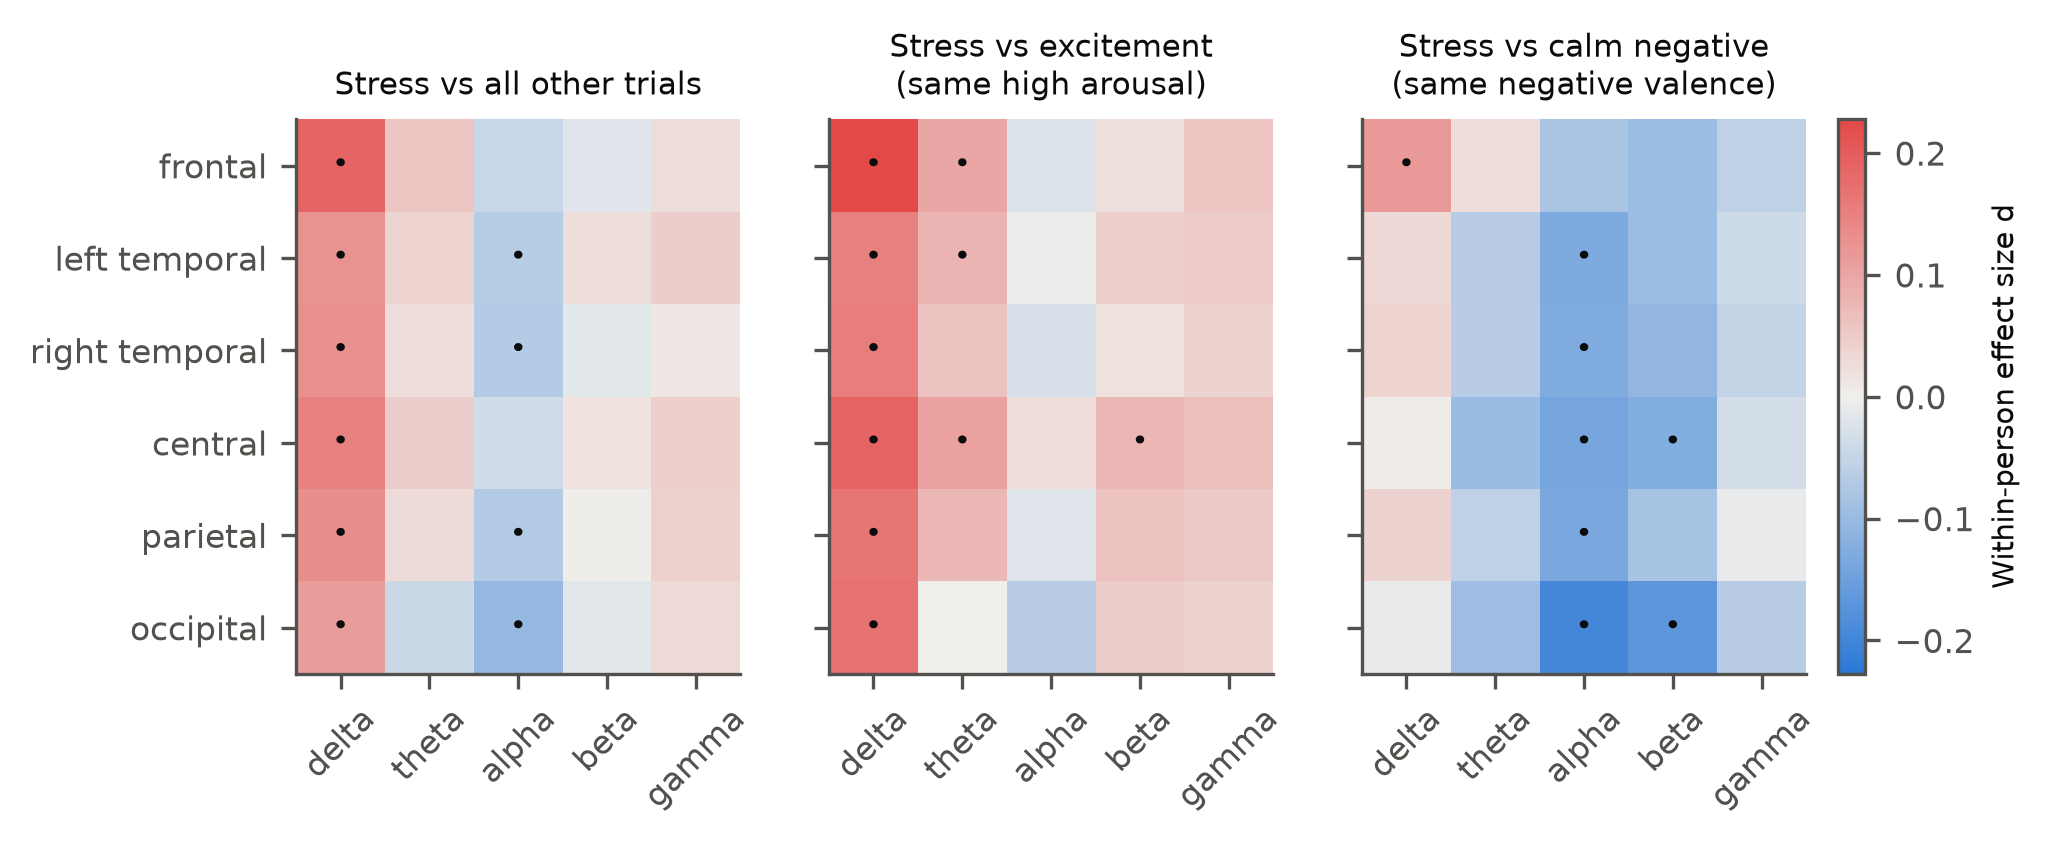
\includegraphics[width=\linewidth]{figures/correlates_eeg.png}
\caption{Within-person effect size $d$ of regional EEG band power, development
data. Red means higher on stressed trials. Dots mark 95\% intervals that
exclude zero.}
\label{fig:eeg}
\end{figure}

\begin{figure}[t]
\centering
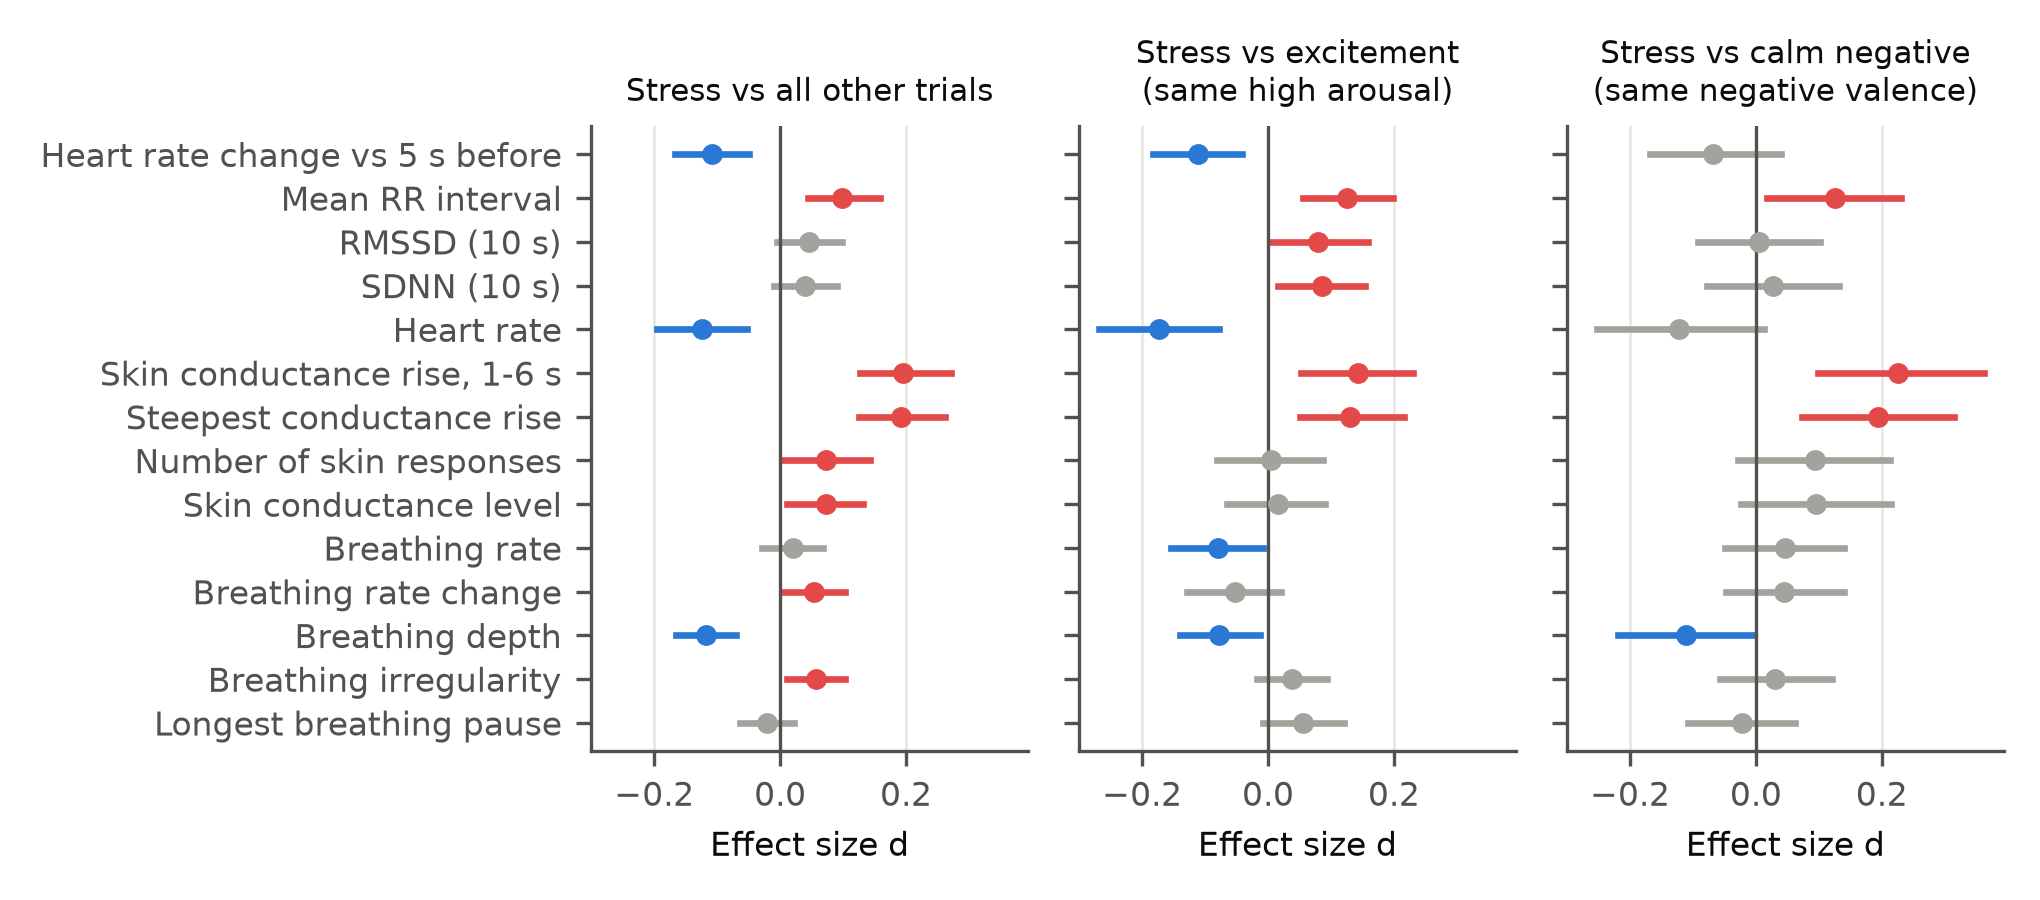
\includegraphics[width=\linewidth]{figures/correlates_body.png}
\caption{Within-person effect size $d$ of heart, skin and breathing features,
development data, with 95\% intervals. Coloured when the interval excludes
zero.}
\label{fig:body}
\end{figure}

\section{What we take from it}

You can detect self-reported stress reactions to short videos from physiology,
in people and videos the model never saw, but only a little: a within-person
AUC around 0.56 to 0.60. A plain logistic regression does as well as the best
model our search produced. The 43-variant search improved the development
score by 0.048, and none of it carried over to the sealed test. In our
previous study on valence and arousal ratings the search gains held; here, with
a binary label, 23\% positives and fewer usable people, they did not. Without a
sealed test we would have reported a better model that does not exist.

The physiology itself is clear and consistent. Stressful videos lower alpha
power, trigger a skin conductance response, make breathing shallower and slow
the heart. For anyone thinking of stress monitoring in practice, the heart
result matters: a short aversive event can lower heart rate, so a detector
that only looks for tachycardia would miss it.

\paragraph{Limitations.} The label is a self-report about a 10-second video in
healthy volunteers, not clinical or chronic stress, and the dataset has no
independent stress measure. The primary test set has 35 usable people, and the
specificity contrasts there rest on 10 to 20 people. The frontal delta
increase may partly be eye movements, since the dataset has no EOG channel and
ICA cleaning is imperfect. Features were fixed before the search, and the final
model rescales its outputs over the batch it predicts, which assumes several
unlabelled trials from the new person.

\paragraph{Reproducibility.} \texttt{decoding/stress.py} holds the scorer,
\texttt{decoding/models/stress.py} the final model and
\texttt{decoding/extract.py} the features.
\nolinkurl{docs/research/stress/experiments.tsv} lists all 43 experiments, and
the sealed numbers and correlates are in \nolinkurl{docs/research/stress/results/}.
Only aggregate numbers are published.

\paragraph{References.} G.~Giannakakis, D.~Grigoriadis, M.~Tsiknakis,
Detection of stress/anxiety state from EEG features during video watching,
IEEE EMBC 2015. HABS team, Stimulus identity rather than emotion drives EEG
classification on the FACED dataset, bioRxiv 10.64898/2026.06.12.731889. M.~M.
Bradley, P.~J.~Lang, emotion and motivation (cardiac deceleration to
unpleasant pictures), in Handbook of Psychophysiology, 2007. HABS team, dataset
paper, 2026.


\end{document}
